\appendix

\chapter{Jira}\label{appendix:jira}
\begin{figure}[h!]
    \centering
    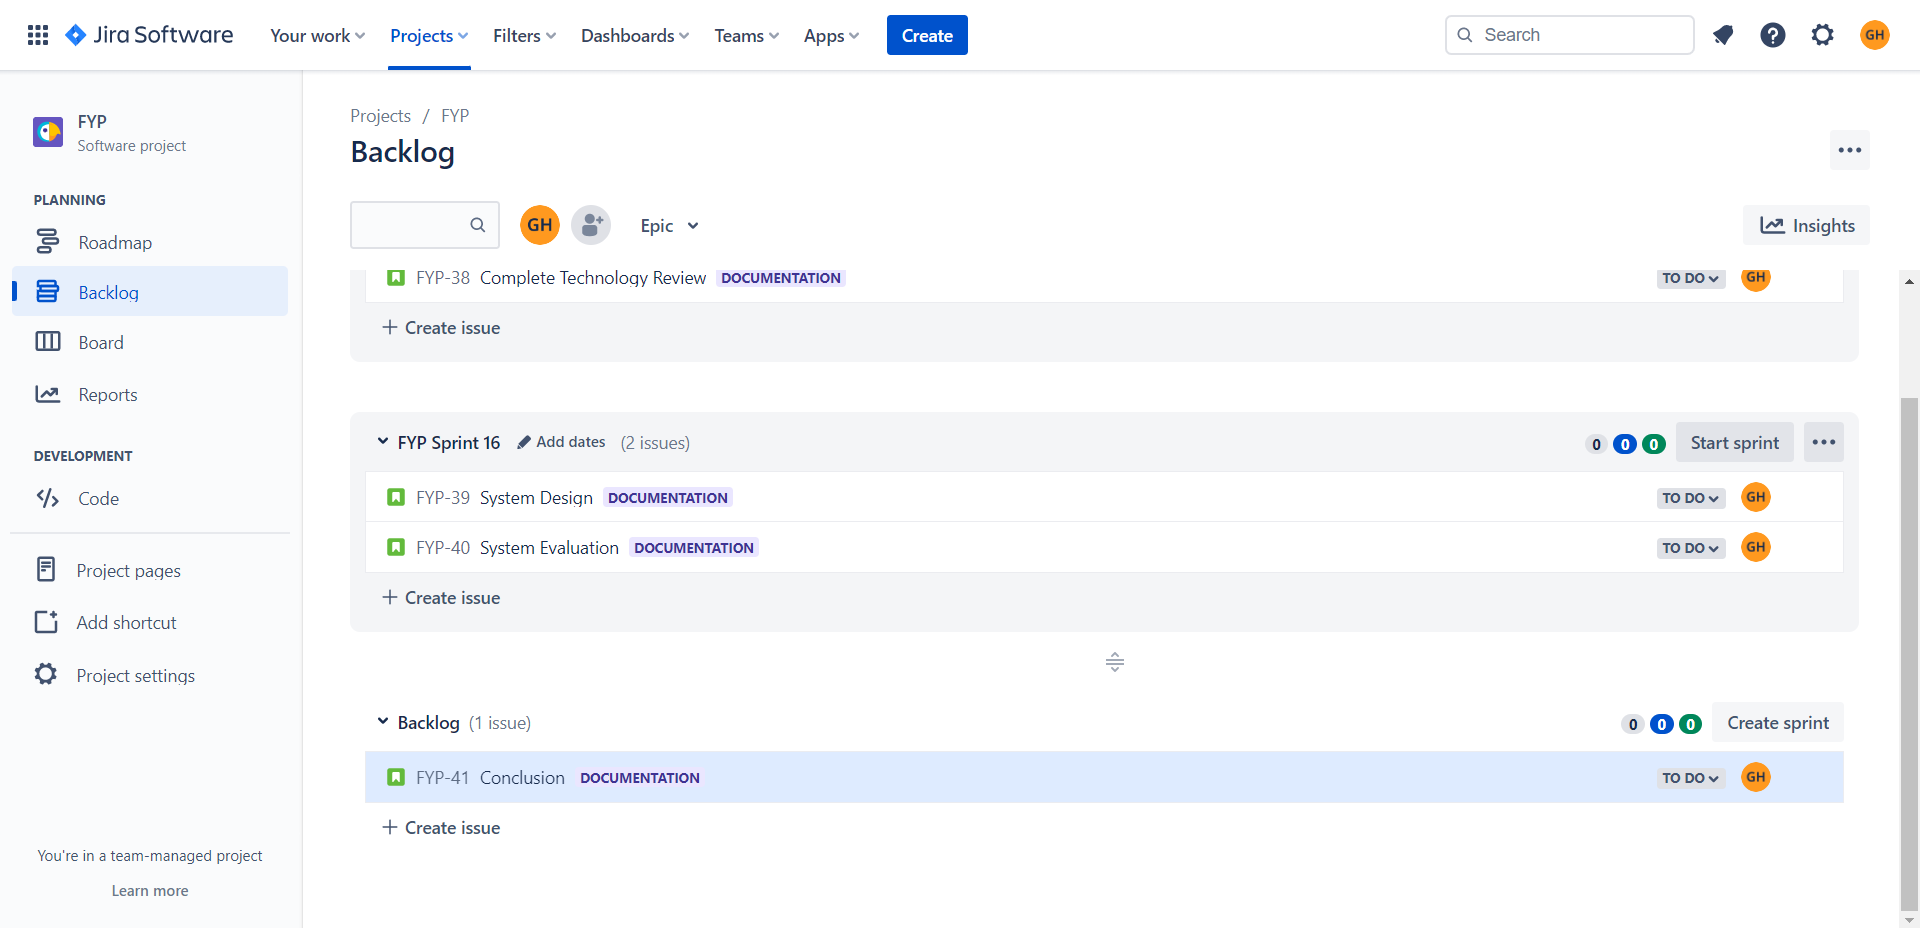
\includegraphics[width=0.9\textwidth]{images/backlog.png}
    \caption{Jira backlog}
    \label{image:backlog}
\end{figure}

\begin{figure}[h!]
    \centering
    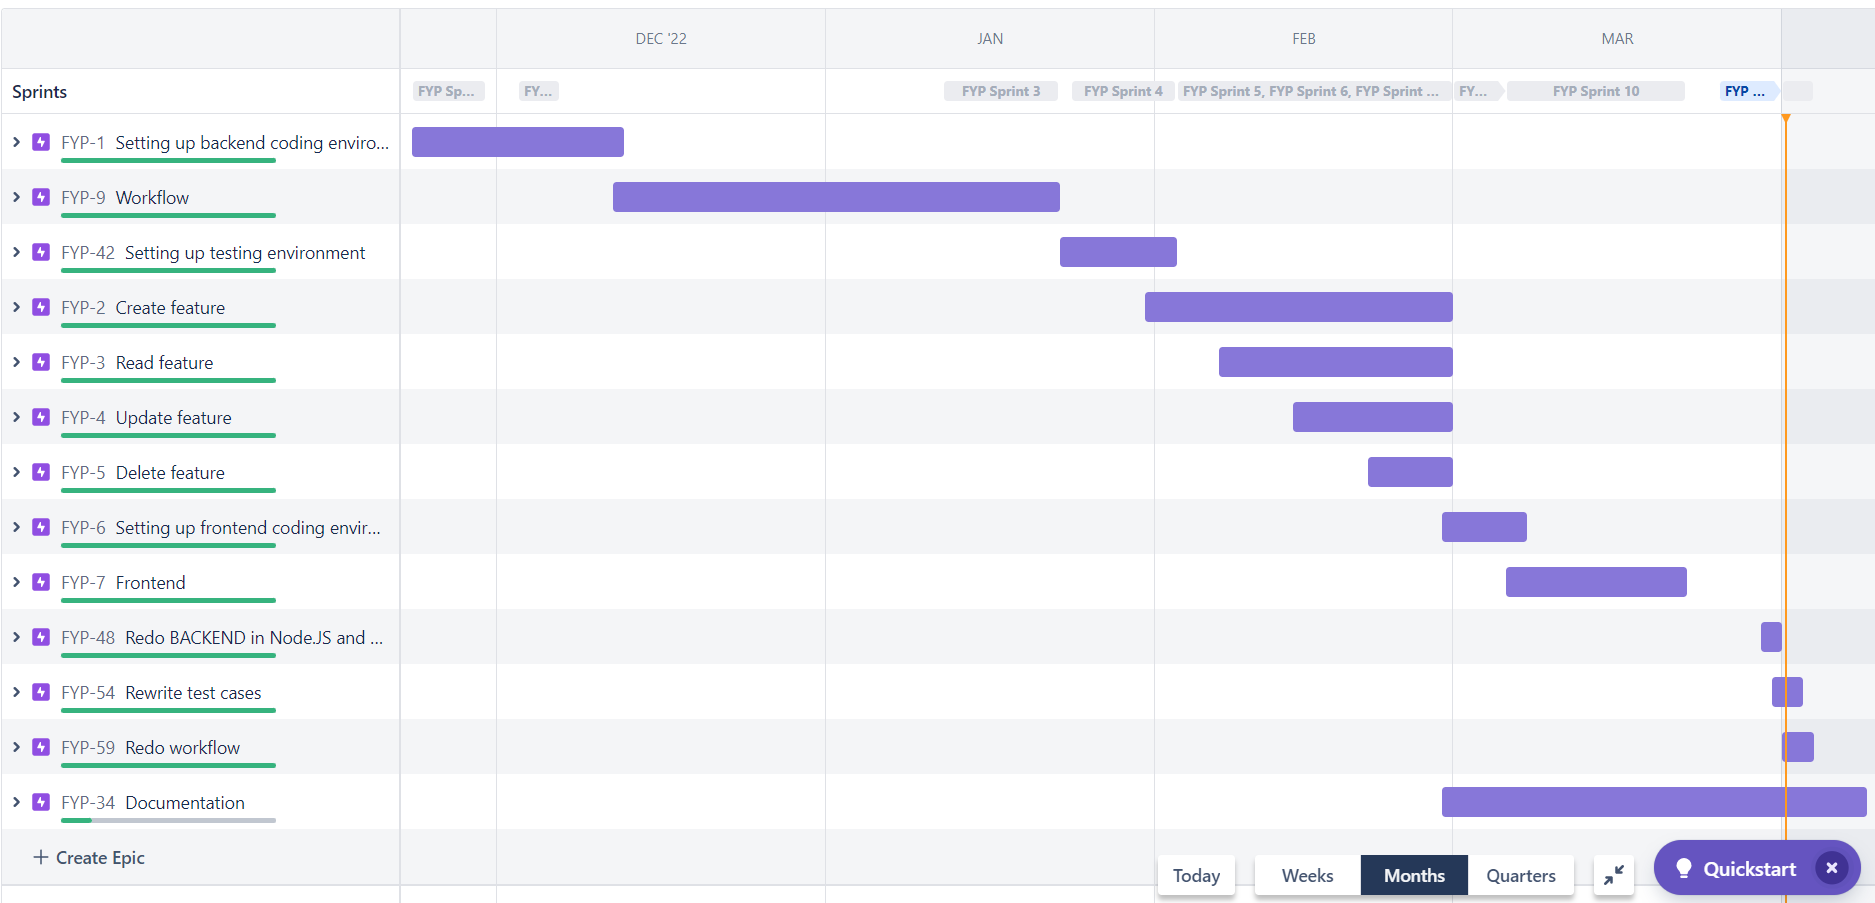
\includegraphics[width=0.9\textwidth]{images/roadmap.png}
    \caption{Jira roadmap}
    \label{image:roadmap}
\end{figure}

\begin{figure}[h!]
    \centering
    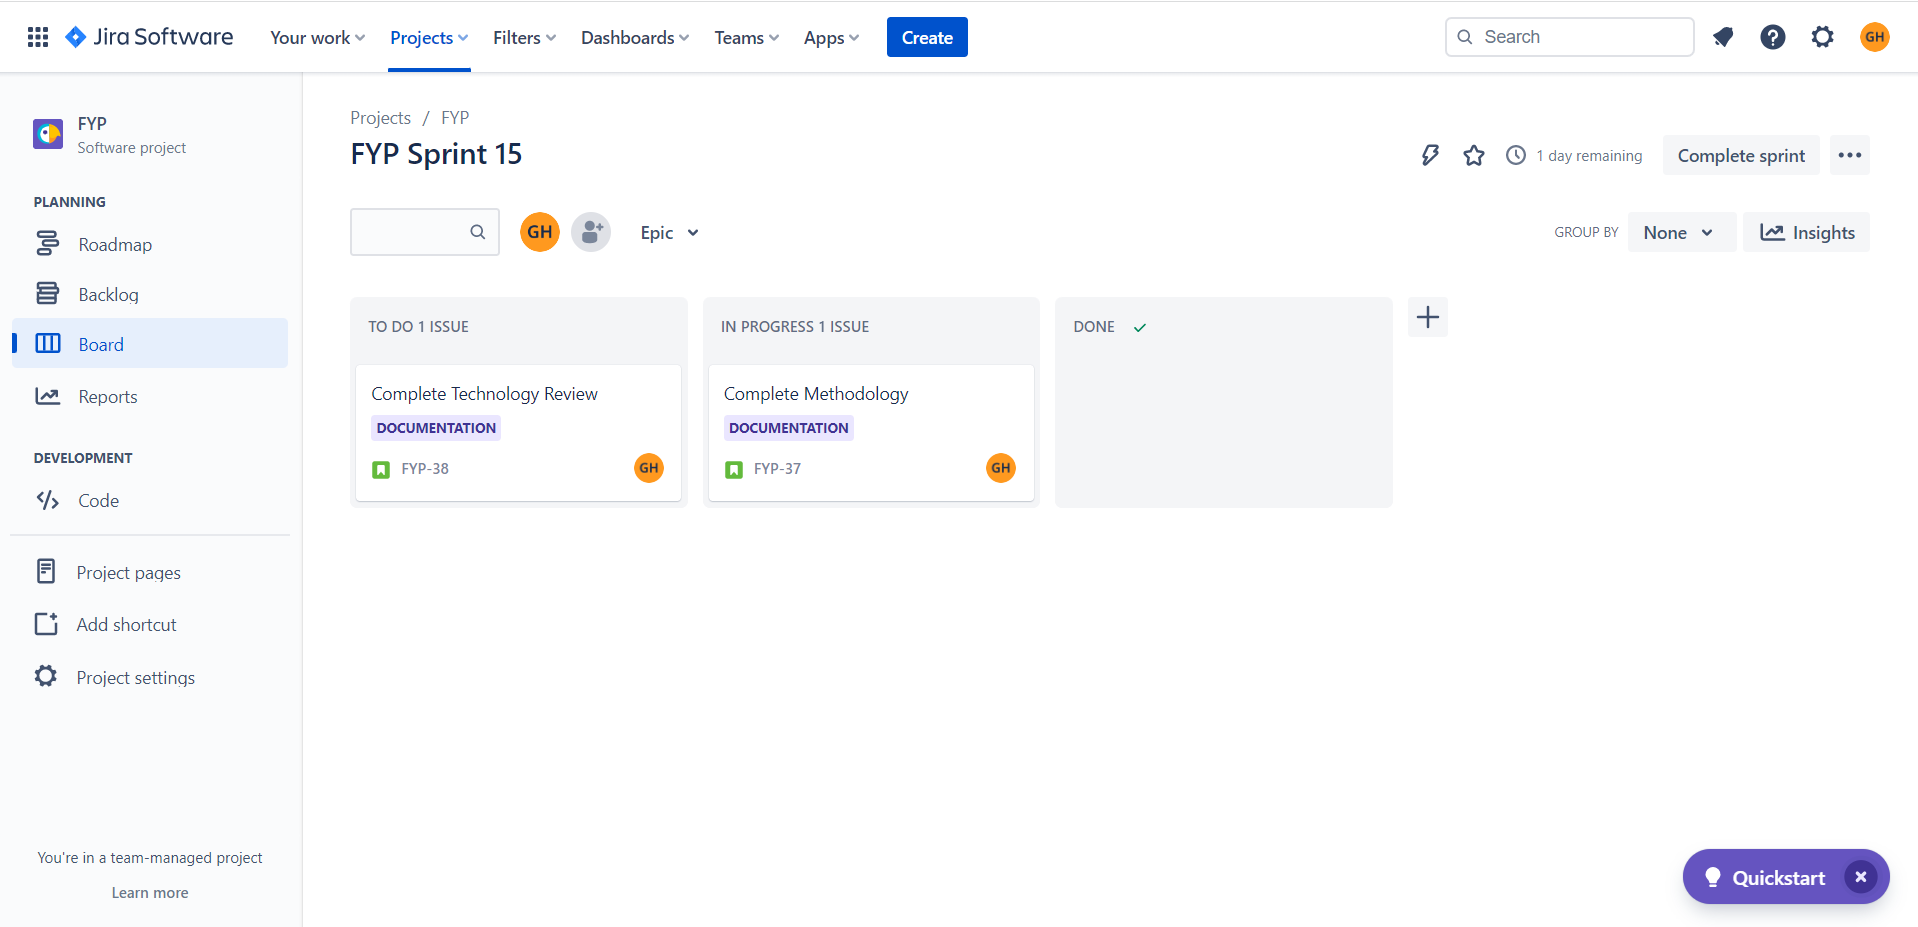
\includegraphics[width=0.9\textwidth]{images/board.png}
    \caption{Jira board}
    \label{image:board}
\end{figure}

\begin{figure}[h!]
    \centering
    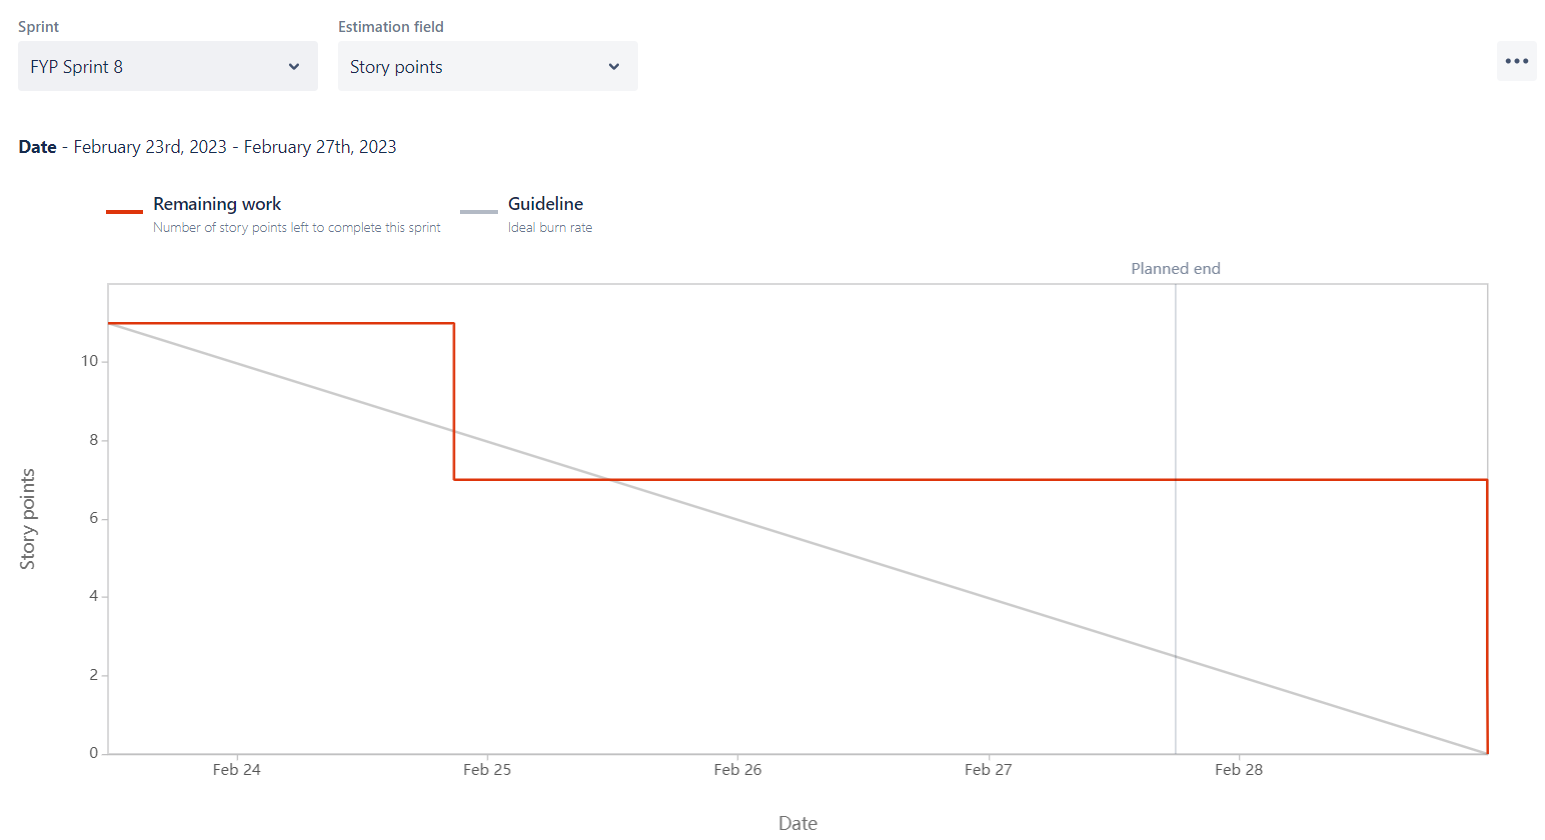
\includegraphics[width=0.9\textwidth]{images/sprint-burndown.png}
    \caption{A Sprint Burndown Chart}
    \label{image:sprint-burndown}
\end{figure}

\chapter{Scrum}\label{appendix:scrum}
\begin{figure}[h!]
    \centering
    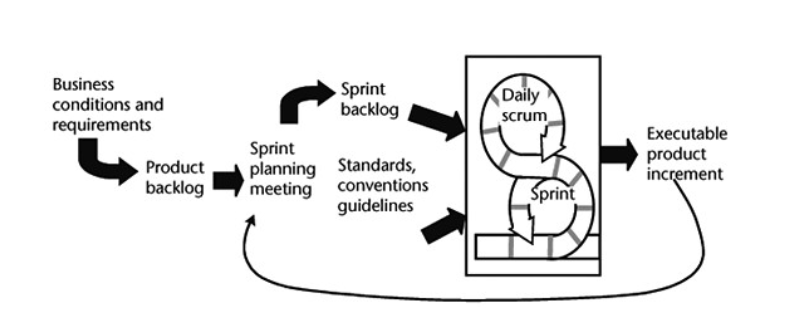
\includegraphics[width=0.9\textwidth]{images/scrum.png}
    \caption{Scrum Process Diagram}
    \label{image:scrum}
\end{figure}

\chapter{DevOps}\label{appendix:devops}
\begin{figure}[h!]
    \centering
    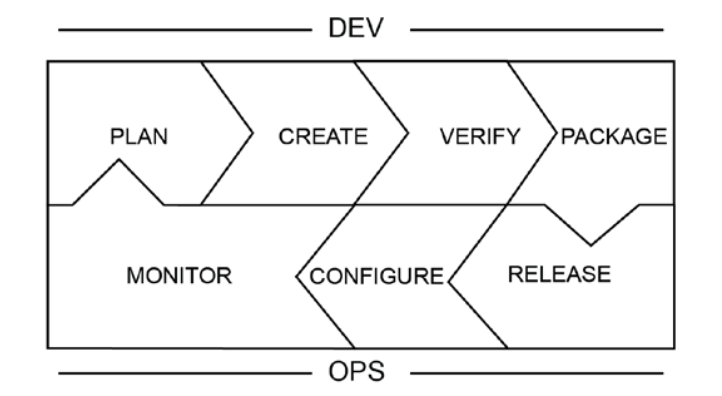
\includegraphics[width=0.9\textwidth]{images/devops.png}
    \caption{The DevOps Toolchain}
    \label{image:devops}
\end{figure}

\begin{figure}[h!]
    \centering
    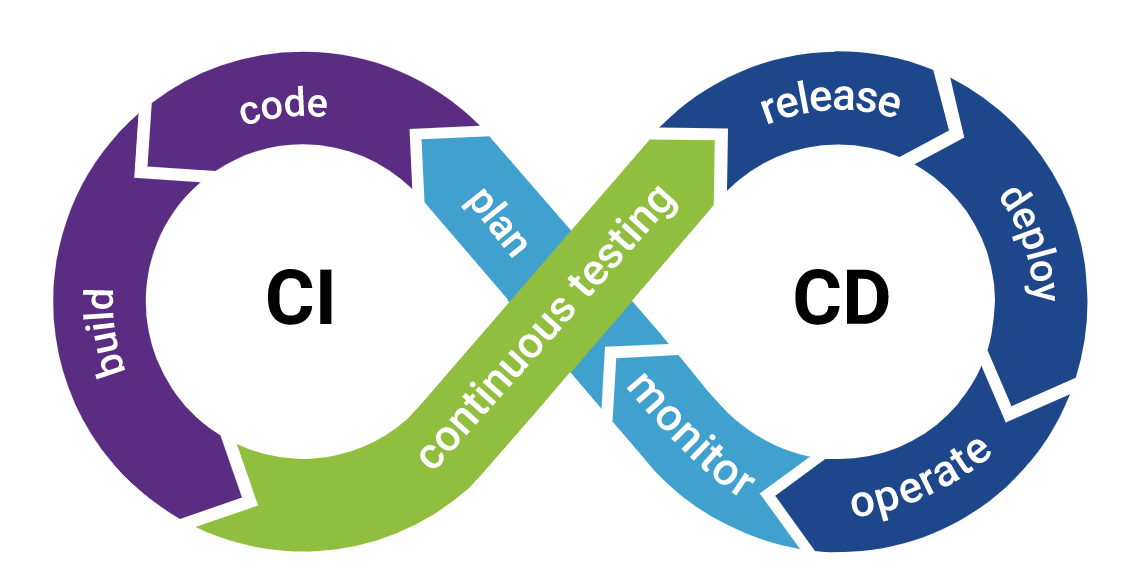
\includegraphics[width=0.9\textwidth]{images/CICD.png}
    \caption{The CI/CD Process}
    \label{image:cicd}
\end{figure}

\chapter{MERN}\label{appendix:mern}
\begin{itemize}
\item MongoDB: A database based on the document-oriented data model.
\item Express.js: A web application framework that allows for the creation of APIs and websites.
\item React.js: A JavaScript library for creating user interfaces that takes a declarative, component-based approach.
\item Node.js: A JavaScript runtime environment that enables the development of platform-independent servers, tools, and applications.
\end{itemize}

\begin{figure}[h!]
    \centering
    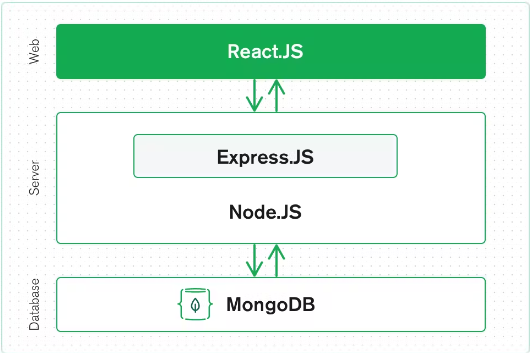
\includegraphics[width=0.9\textwidth]{images/mern.png}
    \caption{The MERN Stack Architecture}
    \label{image:mern}
\end{figure}

\chapter{CI/CD Design and Implementation}\label{appendix:CICD}
\begin{figure}[h!]
    \centering
    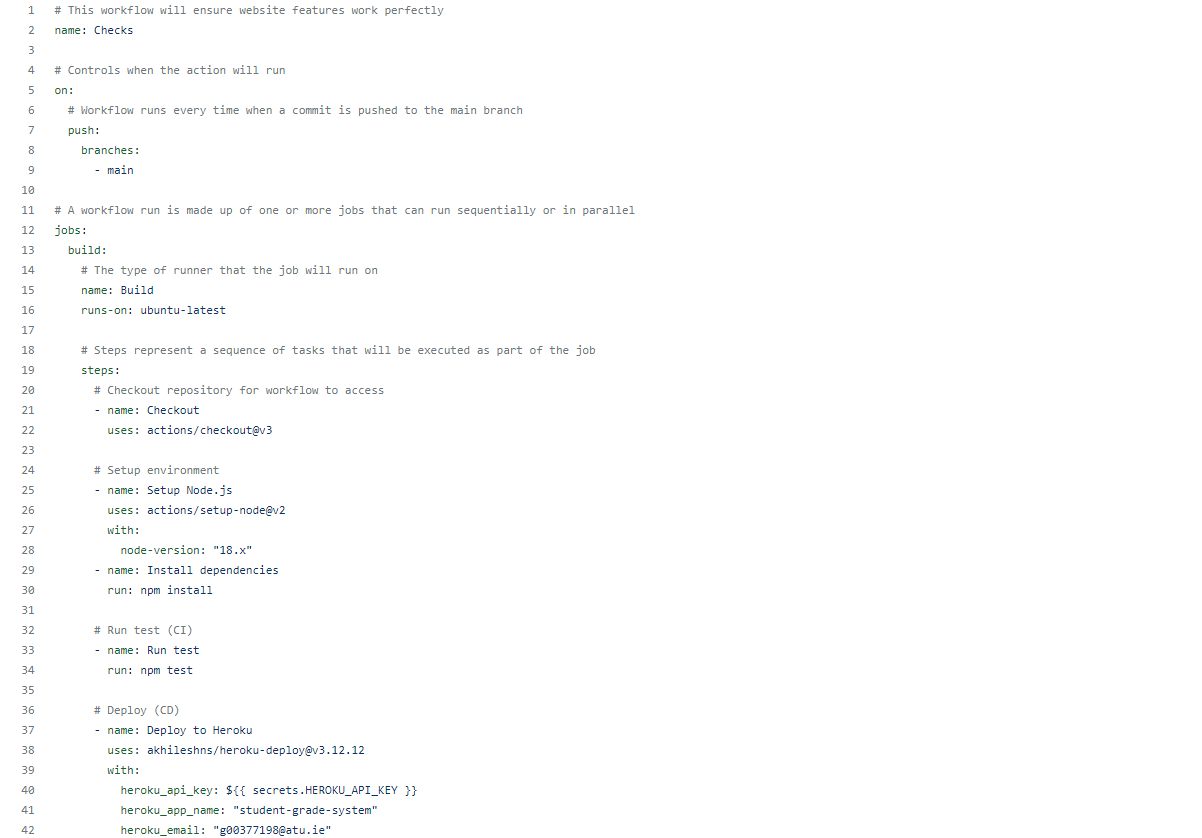
\includegraphics[width=0.9\textwidth]{images/full-workflow.png}
    \caption{GitHub Actions Workflow}
    \label{image:full-workflow}
\end{figure}

\begin{figure}[h!]
    \centering
    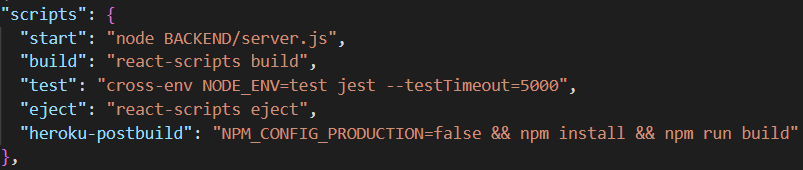
\includegraphics[width=0.9\textwidth]{images/heroku-build.png}
    \caption{Code Snippet from package.json to show heroku-postbuild}
    \label{image:heroku-build}
\end{figure}

\begin{figure}[h!]
    \centering
    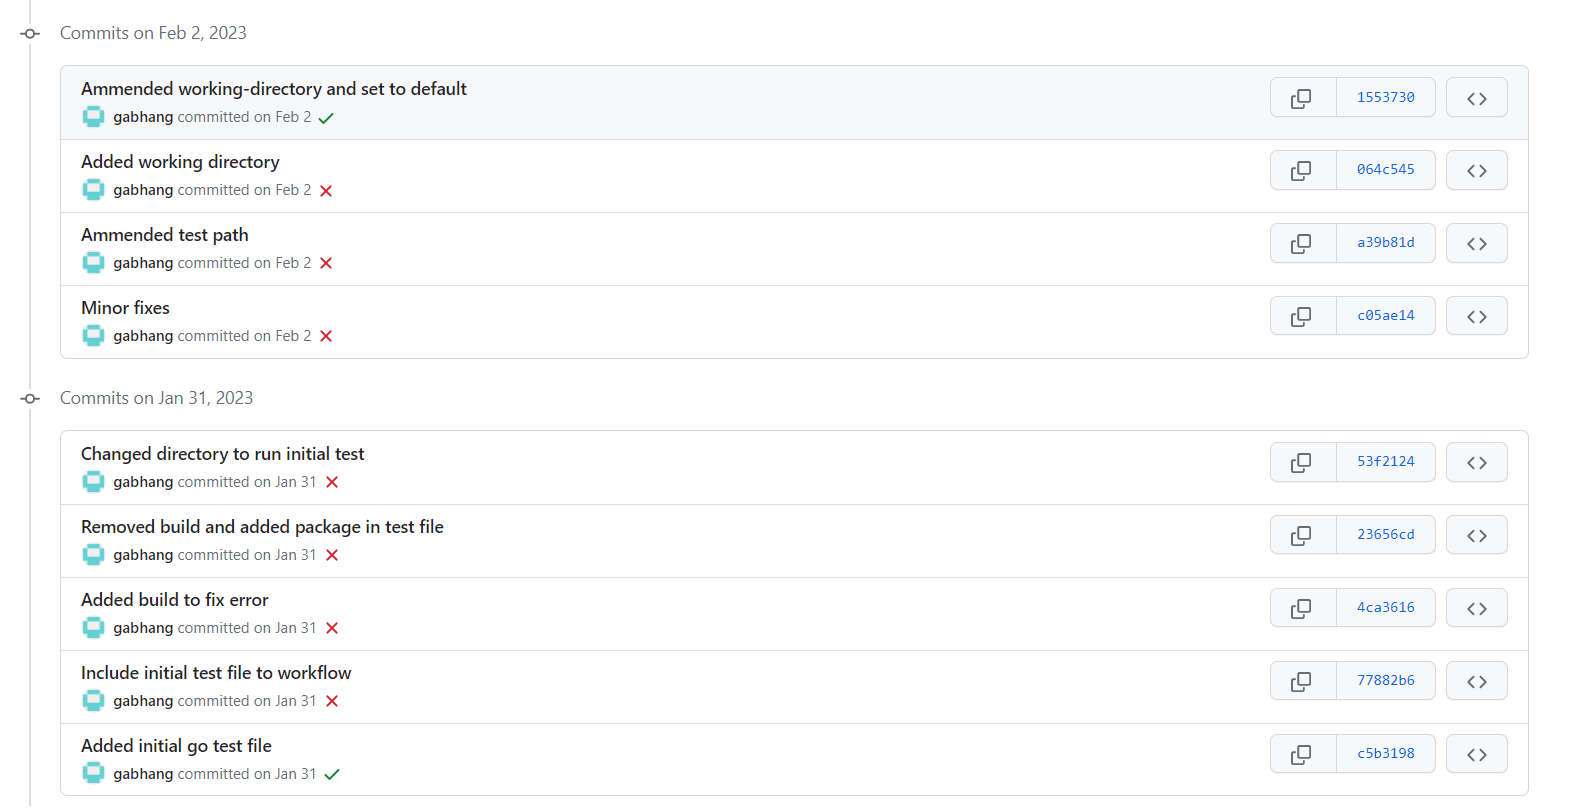
\includegraphics[width=0.9\textwidth]{images/workflow-failed.png}
    \caption{Evidence of mistakes and corrections during workflow design}
    \label{image:workflow-failed}
\end{figure}

\begin{figure}[h!]
    \centering
    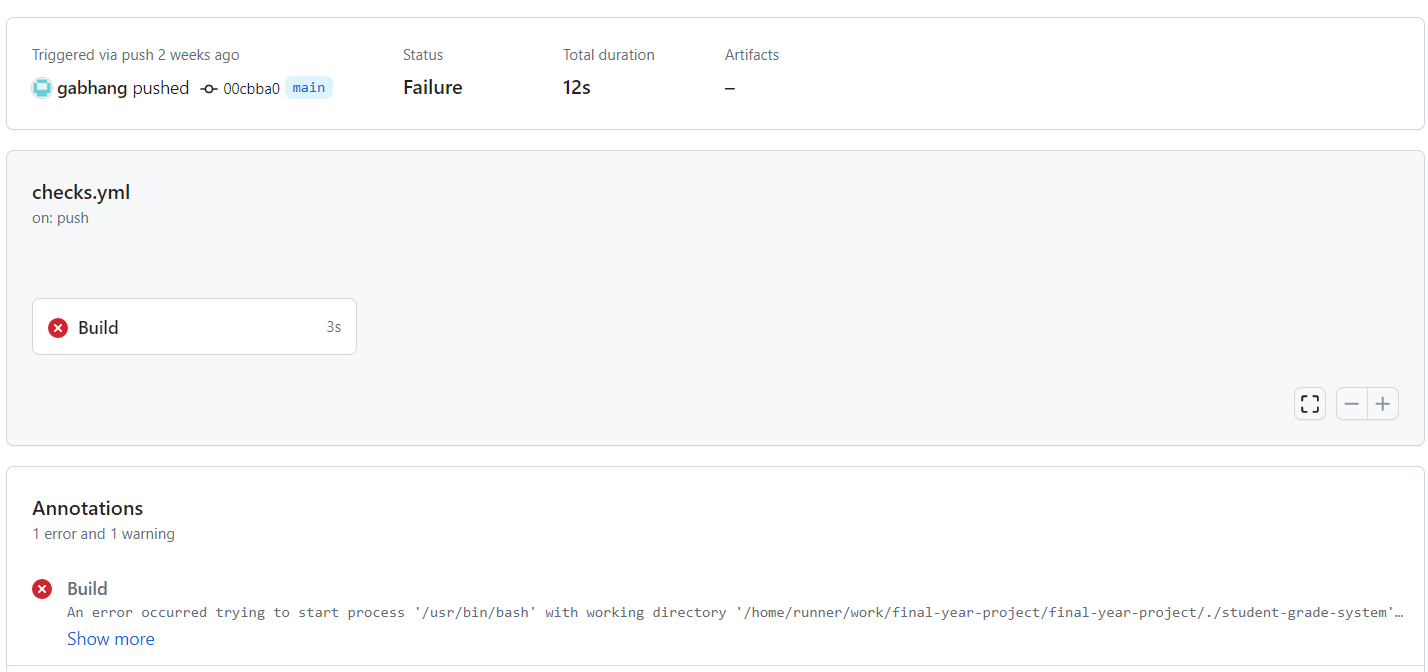
\includegraphics[width=0.9\textwidth]{images/build-fail-directory.png}
    \caption{Directory mismatch error}
    \label{image:build-fail-directory.png}
\end{figure}

\begin{figure}[h!]
    \centering
    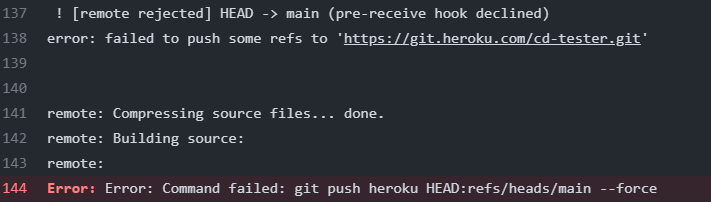
\includegraphics[width=0.9\textwidth]{images/heroku-go-issue.png}
    \caption{Deployment rejection from using GO}
    \label{image:heroku-go-issue.png}
\end{figure}

\begin{figure}[h!]
    \centering
    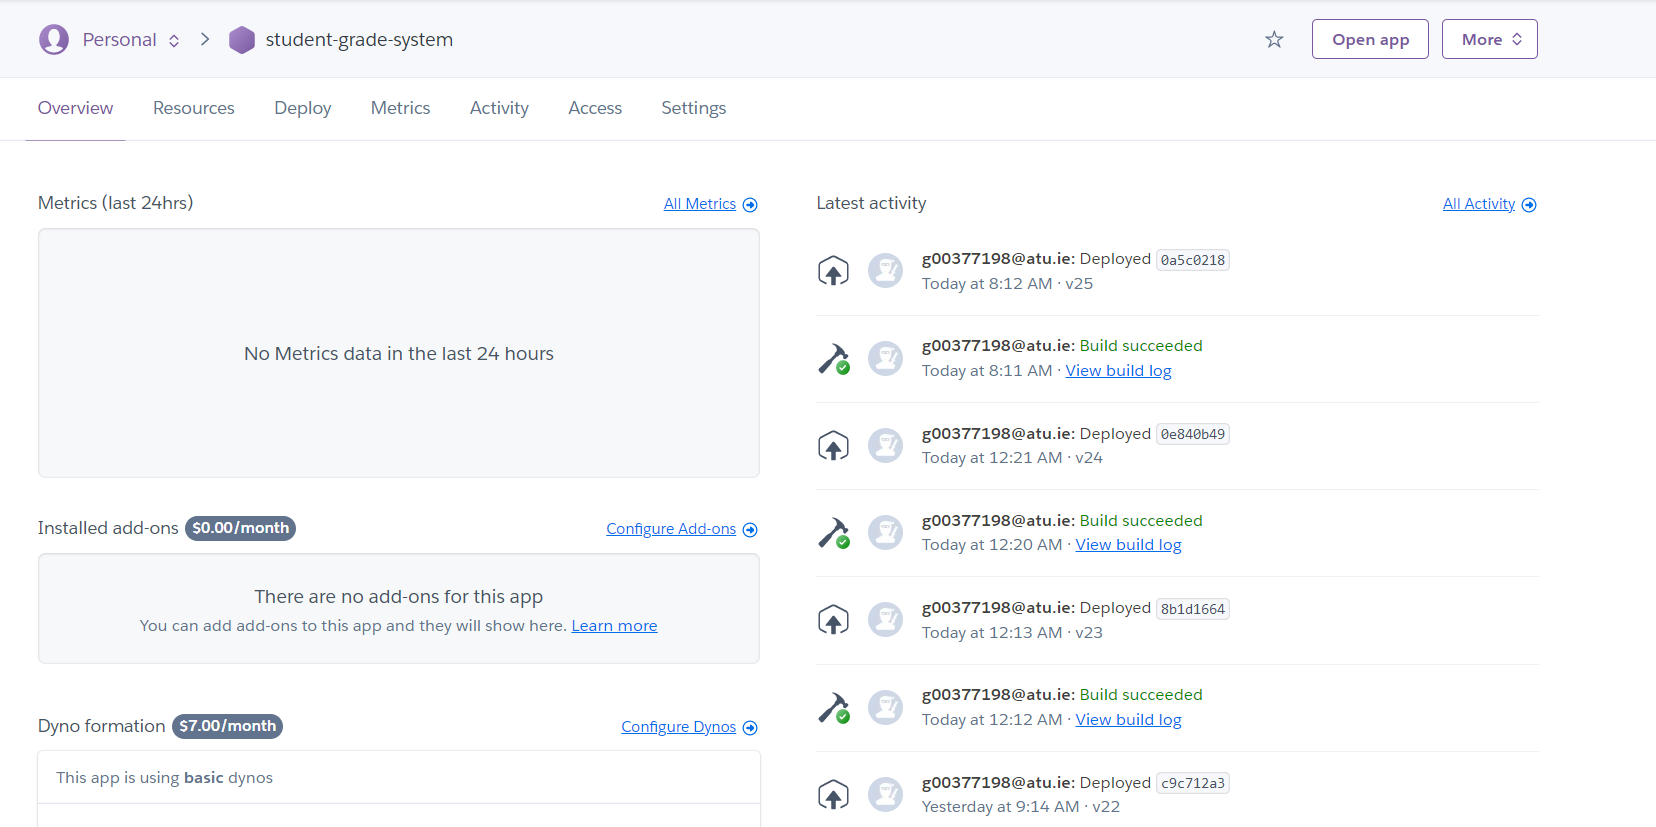
\includegraphics[width=0.9\textwidth]{images/heroku-success.png}
    \caption{Successful deployment in Heroku}
    \label{image:heroku-success.png}
\end{figure}